%\begin{frame}
%\frametitle{Initial Solution: MST}
%\begin{itemize}
%	\item Use Prim's Algorithm with transforming edge costs
%	\item Costs depend on already used edges (8-Port Switches)
%	\item 
%\end{itemize}
%\end{frame}

\begin{frame}
  \begin{center}
    \LARGE Heuristic: Minimum Spanning Tree (MST)
  \end{center}
\end{frame}

%\begin{frame}
%\frametitle{MST Initial}
%\begin{adjustbox}{max width=0.9\paperwidth,center}
%	\begin{tikzpicture}[node distance=2cm]
%	\tikzstyle{vertex}=[draw,shape=circle, minimum size=1cm];
%	\node[vertex] (A){A};
%	\node[node distance=0.5cm] (left)[left=of A]{};
%	\node[vertex] (B) [right=1.5cm of A] {B};
%	\node[vertex] (C) [above= 1cm of B] {C};
%	\node[vertex] (X) [right=4.5cm of B] {X};
%	
%	\draw[line width=0.55mm,black] (A) -- (left);
%	\draw[line width=0.55mm,black] (A) -- (B);
%	\draw[line width=0.55mm,black] (B) -- (C);
%	
%	\end{tikzpicture}
%\end{adjustbox}
%\end{frame}

\begin{frame}
\frametitle{Initial Solution: MST}
\begin{figure}
\begin{adjustbox}{max width=0.9\paperwidth,center}
	\begin{tikzpicture}[node distance=2cm]
	\tikzstyle{vertex}=[draw,shape=circle, minimum size=1cm];
	\node[vertex] (A){A};
	\node[node distance=0.5cm] (left)[left=of A]{};
	\node[vertex] (B) [right=1.5cm of A] {B};
	\node[vertex] (C) [above= 1cm of B] {C};
	\node[vertex] (X) [right=4.5cm of B] {X};
	
	\draw[line width=0.55mm,black] (A) -- (left);
	\draw[line width=0.55mm,black] (A) -- (B);
	\draw[line width=0.55mm,black] (B) -- (C);
	
	\draw[line width=0.30mm,orange,dashed] (B) -- node[below] {\small  Distance \textcolor{black}{$+$} \textcolor{blue}{LOC Costs}} (X);
	%\draw[line width=0.30mm,blue, transform canvas={yshift=-1cm},shorten >= 1.2cm, shorten <=1.2cm] (B) -- node[below] {\small LOC} (X);
	\draw[line width=0.30mm, orange,dashed] (C) -- node[above, sloped] {\small Distance} (X);
	\end{tikzpicture}
\end{adjustbox}
\caption{Include switch installation into edge costs.}
\end{figure}
\end{frame}



%\begin{frame}
%\frametitle{Local Search: Spanning Tree}
%\begin{itemize}
%	\item Delete Edge
%	\item x
%	\item z
%\end{itemize}
%\end{frame}
\begin{frame}
\frametitle{Local Search: Cycle Neighborhood}
\begin{figure}
\begin{adjustbox}{max width=0.9\paperwidth,center}
	\begin{tikzpicture}[node distance=1cm]
	\tikzstyle{vertex}=[draw,shape=circle, minimum size=1cm];
	\tikzstyle{partition}=[draw, minimum width=4cm, minimum height=1.5cm, shape=rectangle];
	\node[vertex] (T){T};
	\node[partition] (P1) [above=of T] {$P_1$};
	\node[partition] (P2) [above=of P1] {$P_2$};
	
	\draw[line width=0.55mm,black] (T) -- (P1);
	\draw[line width=0.55mm,black, transform canvas={xshift=-1cm}] (P1) -- node[strike out,draw, red]{} node[right] {\small e} (P2);
	\draw[line width=0.55mm,blue, transform canvas={xshift=1cm}] (P1) -- node[right] {\small f} (P2);
	\end{tikzpicture}
\end{adjustbox}
\caption{Consider the cycle neighborhood, that is, delete edge $e$ and reconnect the resulting partitions $P_1$ and $P_2$ by adding an edge $f$ with $c(f) < c(e)$.}
\end{figure}
\end{frame}
\begin{frame}
\frametitle{Local Search: Cycle Neighborhood - Power Cables}
\begin{figure}
  \begin{adjustbox}{max width=0.9\paperwidth, max height=0.5\paperwidth,center}
    \begin{tikzpicture}[node distance=1cm]
    \tikzstyle{vertex}=[draw,shape=circle, minimum size=0.7cm];
    \node[vertex] (T){T};
    \node[vertex,fill,blue] (p1)[above left=1cm and 4cm of T]{};
    \node[vertex,fill,blue] (p2)[above left=1cm and 2cm of p1]{};
    \node[vertex,fill,blue] (p3)[above right=0.5cm and 2cm of p2]{};
    \node[vertex,fill,orange] (q1)[above right=1cm and 4cm of T]{};
    \node[vertex,fill,orange] (q2)[above right=1cm and 2cm of q1]{};
    \node[vertex,fill,orange] (q3)[above left=1cm and 3cm of q2]{};
    
    \node[vertex] (v)[above right=1cm and 2cm of p3]{v};
    \node[vertex] (w)[above left=1cm and 2.5cm of q3]{w};
    \node[vertex,fill=black!60!green] (n1)[above right=0.3cm and 0.5 of w]{};
    
    \draw[line width=0.55mm, decorate,decoration={snake,post length=1mm}, ->] (T) -- (p1);
    \draw[line width=0.55mm, ->] (p1) -- (p2);
    \draw[line width=0.55mm, ->] (p2) -- (p3);
    \draw[line width=0.55mm, ->] (p3) -- (v);
    
    
    \draw[line width=0.55mm, decorate,decoration={snake,post length=1mm}, ->] (T) -- (q1);
    \draw[line width=0.55mm, ->] (q1) -- (q2);
    \draw[line width=0.55mm, ->] (q2) -- (q3);
    \draw[line width=0.55mm, ->] (q3) -- node[strike out,draw, red]{} (w);
    
    \draw[line width=0.55mm, ->] (w) -- (n1);
    
    \draw[line width=0.55mm, ->,dashed] (v) -- (w);
    
    \matrix [left=1cm of v]  {
      \node[label=right:Sucessors of $w$, vertex,fill=black!60!green,minimum size=0.3cm] [] {}; \\
      \node[label=right:Parents of $w$, vertex,fill,orange,minimum size=0.3cm] {}; \\
      \node[label=right:Parents of $v$, vertex,fill,blue,minimum size=0.3cm] {}; \\	
    };
    
    \node (l1) [above right=3pt of q3] {Path};
    \node (l2) [right=of l1] {};
    \node (l3) [above=5pt of l2] {};
    \node (l4) [left=of l3] {Delete edge};
    \node (l5) [above=5pt of l3] {};
    \node (l6) [left=of l5] {Add edge};
    \draw[line width=0.55mm, decorate,decoration={snake,post length=1mm}, ->] (l1) -- (l2);
    \draw[line width=0.55mm, ->] (l4) -- node[strike out,draw, red]{} (l3);
    \draw[line width=0.55mm, ->,dashed] (l6) -- (l5);
    
    \end{tikzpicture}
  \end{adjustbox}
  \caption{For power cables we need to consider up- and downgrades regarding cables $\Rightarrow$ potential savings by switching to lower-quality cables.}
\end{figure}
\end{frame}

\begin{frame}
\frametitle{Local Search: Cycle Neighborhood - Power Cables}
\begin{figure}
\begin{adjustbox}{max width=0.9\paperwidth, max height=0.5\paperwidth,center}
  \begin{tikzpicture}[node distance=1cm]
  \tikzstyle{vertex}=[draw,shape=circle, minimum size=0.7cm];
  \node[vertex] (T){T};
  \node[vertex,fill=black] (p1)[above left=1cm and 4cm of T]{};
  \node[vertex,fill=black] (p2)[above left=1cm and 2cm of p1]{};
  \node[vertex,fill=black] (p3)[above right=0.5cm and 2cm of p2]{};
  \node[vertex,fill=black] (q1)[above right=1cm and 4cm of T]{};
  \node[vertex,fill=black] (q2)[above right=1cm and 2cm of q1]{};
  \node[vertex,fill=black] (q3)[above left=1cm and 3cm of q2]{};
  
  \node[vertex] (v)[above right=1cm and 2cm of p3]{v};
  \node[vertex] (w)[above left=1cm and 2.5cm of q3]{w};
  \node[vertex,fill=black] (n1)[above right=0.3cm and 0.5 of w]{};
  
  \draw[line width=0.55mm, decorate,decoration={snake,post length=1mm}, ->] (T) -- (p1);
  \draw[line width=0.55mm, ->] (p1) -- (p2);
  \draw[line width=0.55mm, ->] (p2) -- (p3);
  \draw[line width=0.55mm, ->] (p3) -- (v);
  
  
  \draw[line width=0.55mm, decorate,decoration={snake,post length=1mm}, ->] (T) -- (q1);
  \draw[line width=0.55mm, ->] (q1) -- (q2);
  \draw[line width=0.55mm, ->] (q2) -- (q3);
  
  \draw[line width=0.55mm, ->] (w) -- (n1);
  
  \draw[line width=0.55mm, ->] (v) -- (w);
  \end{tikzpicture}
\end{adjustbox}
\end{figure}
\end{frame}




\begin{frame}
  \begin{figure}
    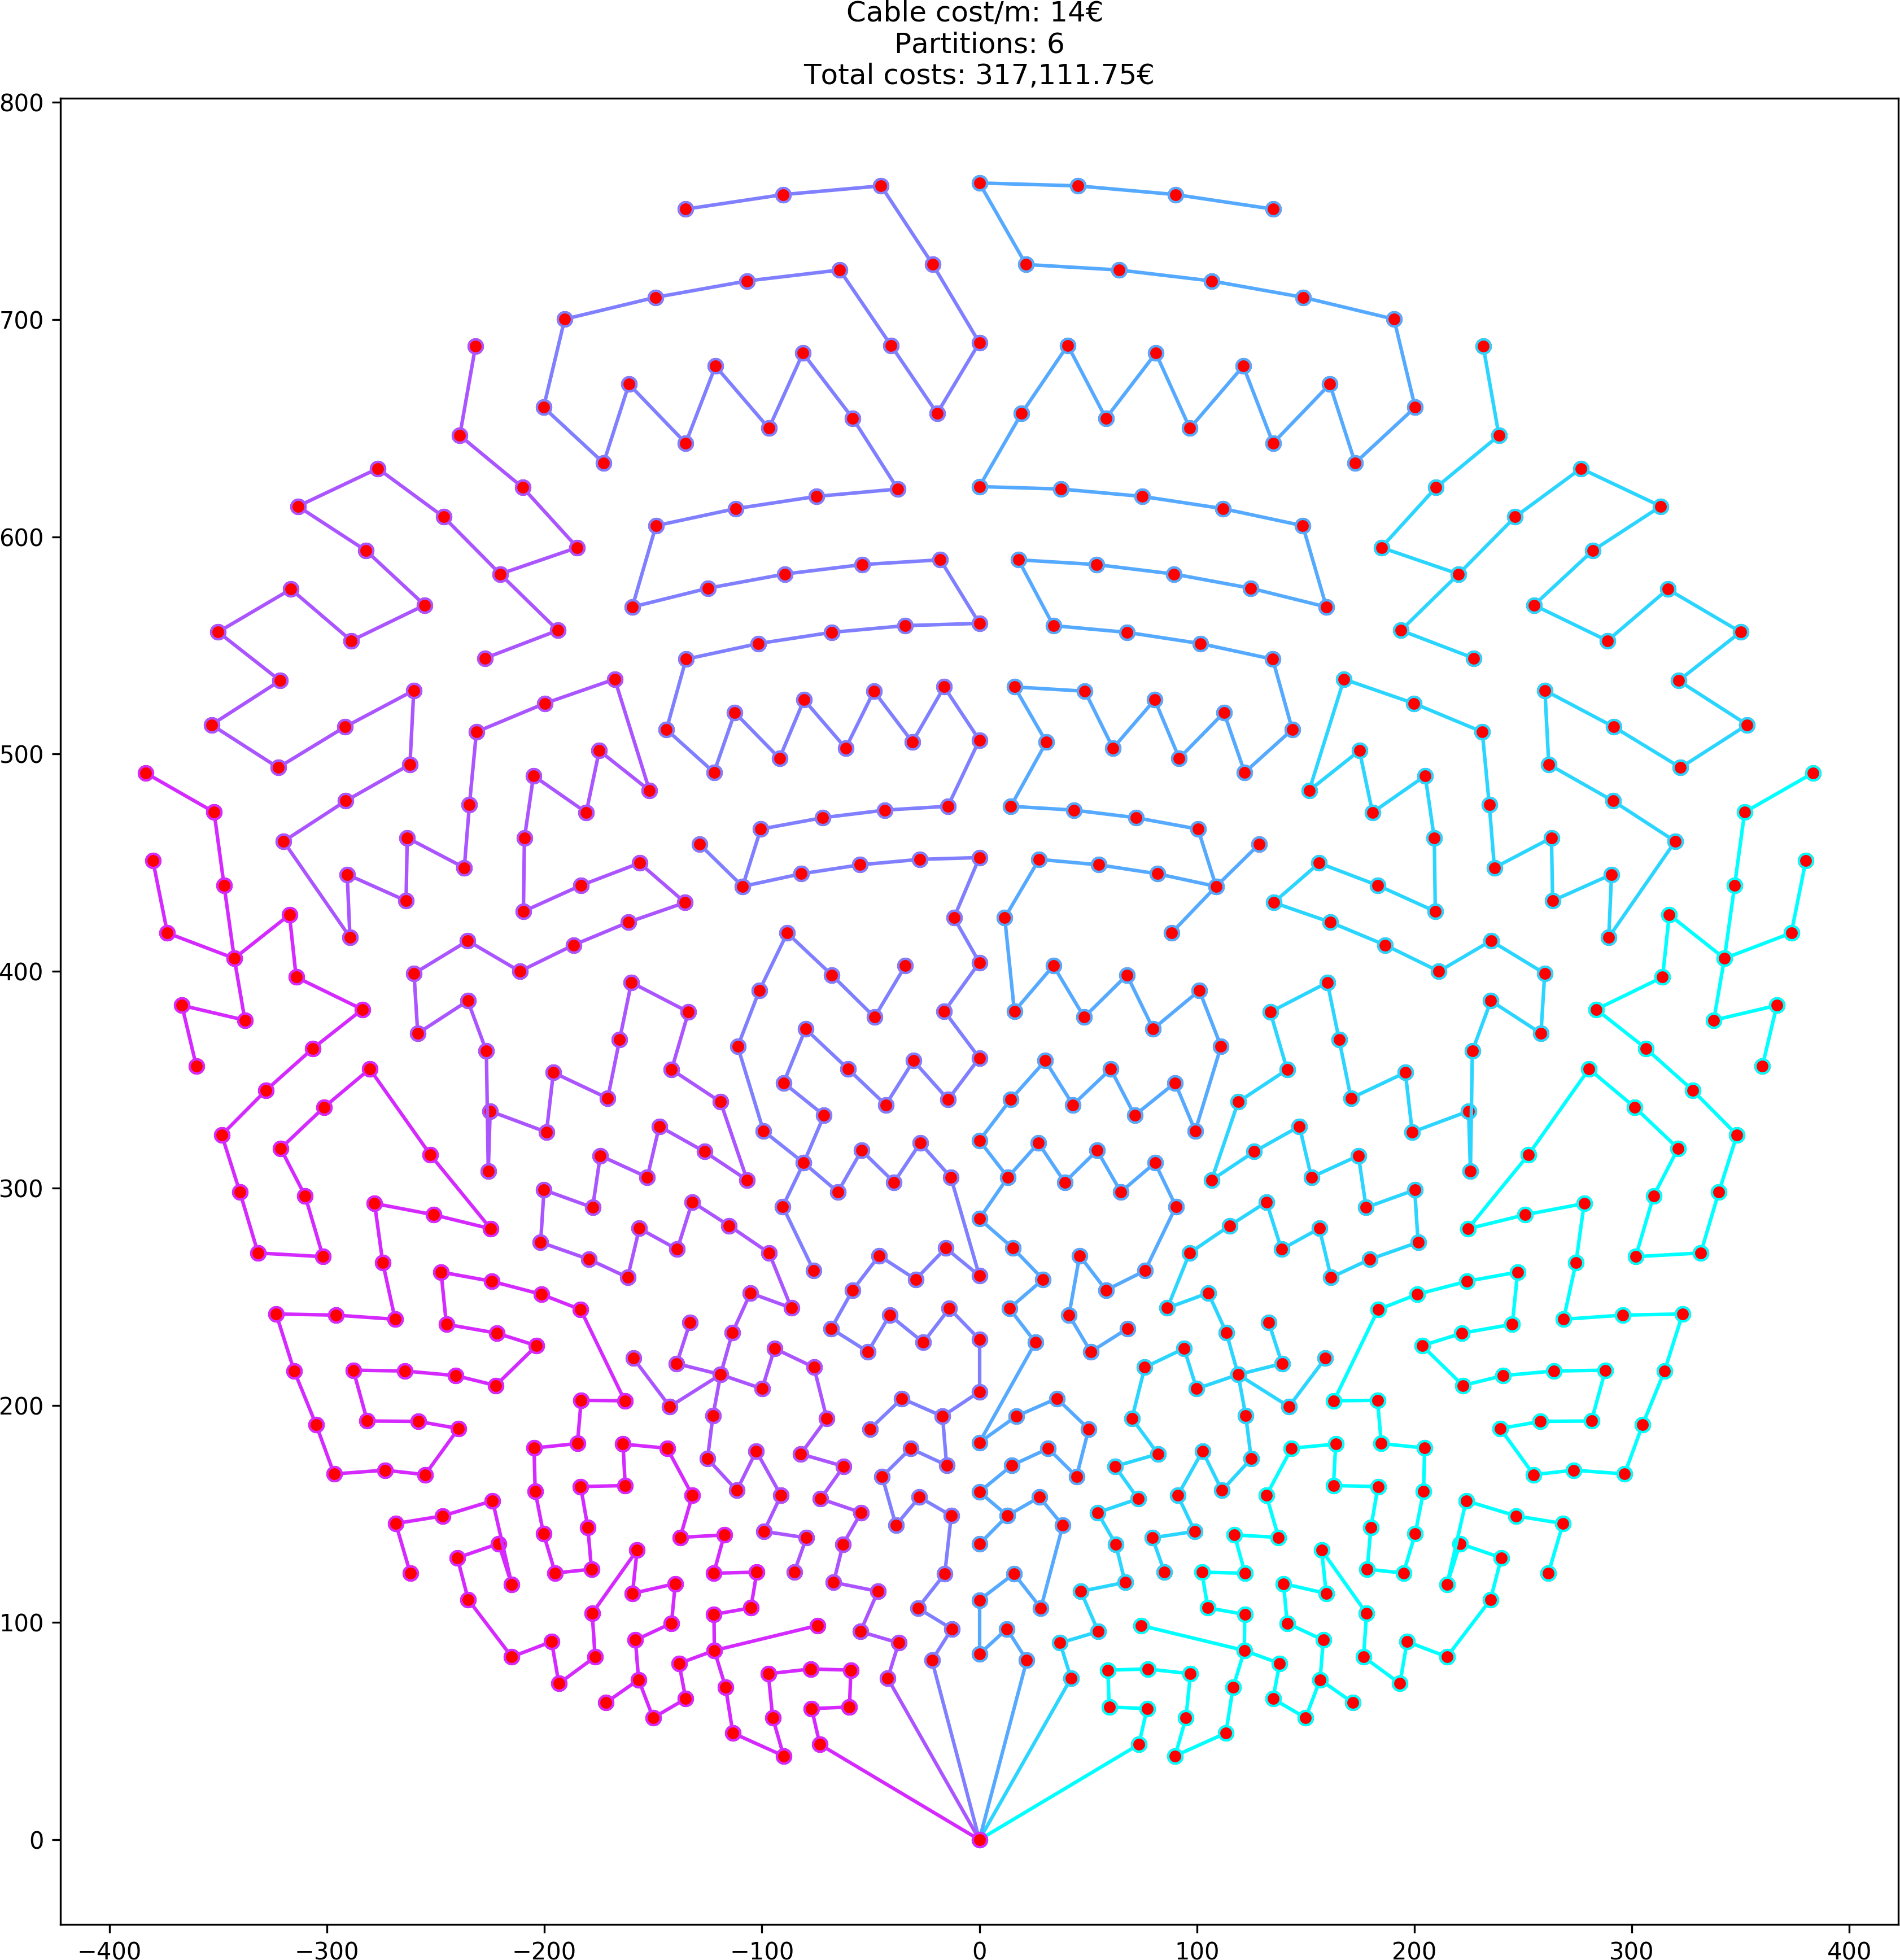
\includegraphics[width=0.75\textwidth]{./figs/init_output_mst_14_6.png}
    \caption{Initial MST solution. Total costs: 317,311.75\euro.}
  \end{figure}
\end{frame}

\begin{frame}{Cycle Neighborhood Improvement}
  \begin{figure}
    \captionsetup[subfigure]{justification=centering}
    \begin{subfigure}{0.45\textwidth}
      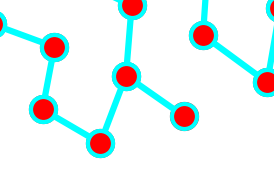
\includegraphics[width=0.75\textwidth]{./figs/init_output_mst_14_6__SELECTION.png}
      \caption{Initial solution.}
    \end{subfigure}
    \begin{subfigure}{0.45\textwidth}
      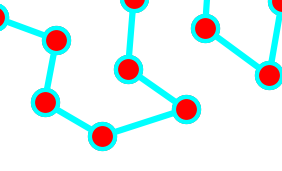
\includegraphics[width=0.75\textwidth]{./figs/output_mst_14_6_SELECTION.png}
      \caption{After cycle improvement.}
    \end{subfigure}
  \end{figure}
\end{frame}

\begin{frame}
  \begin{figure}
    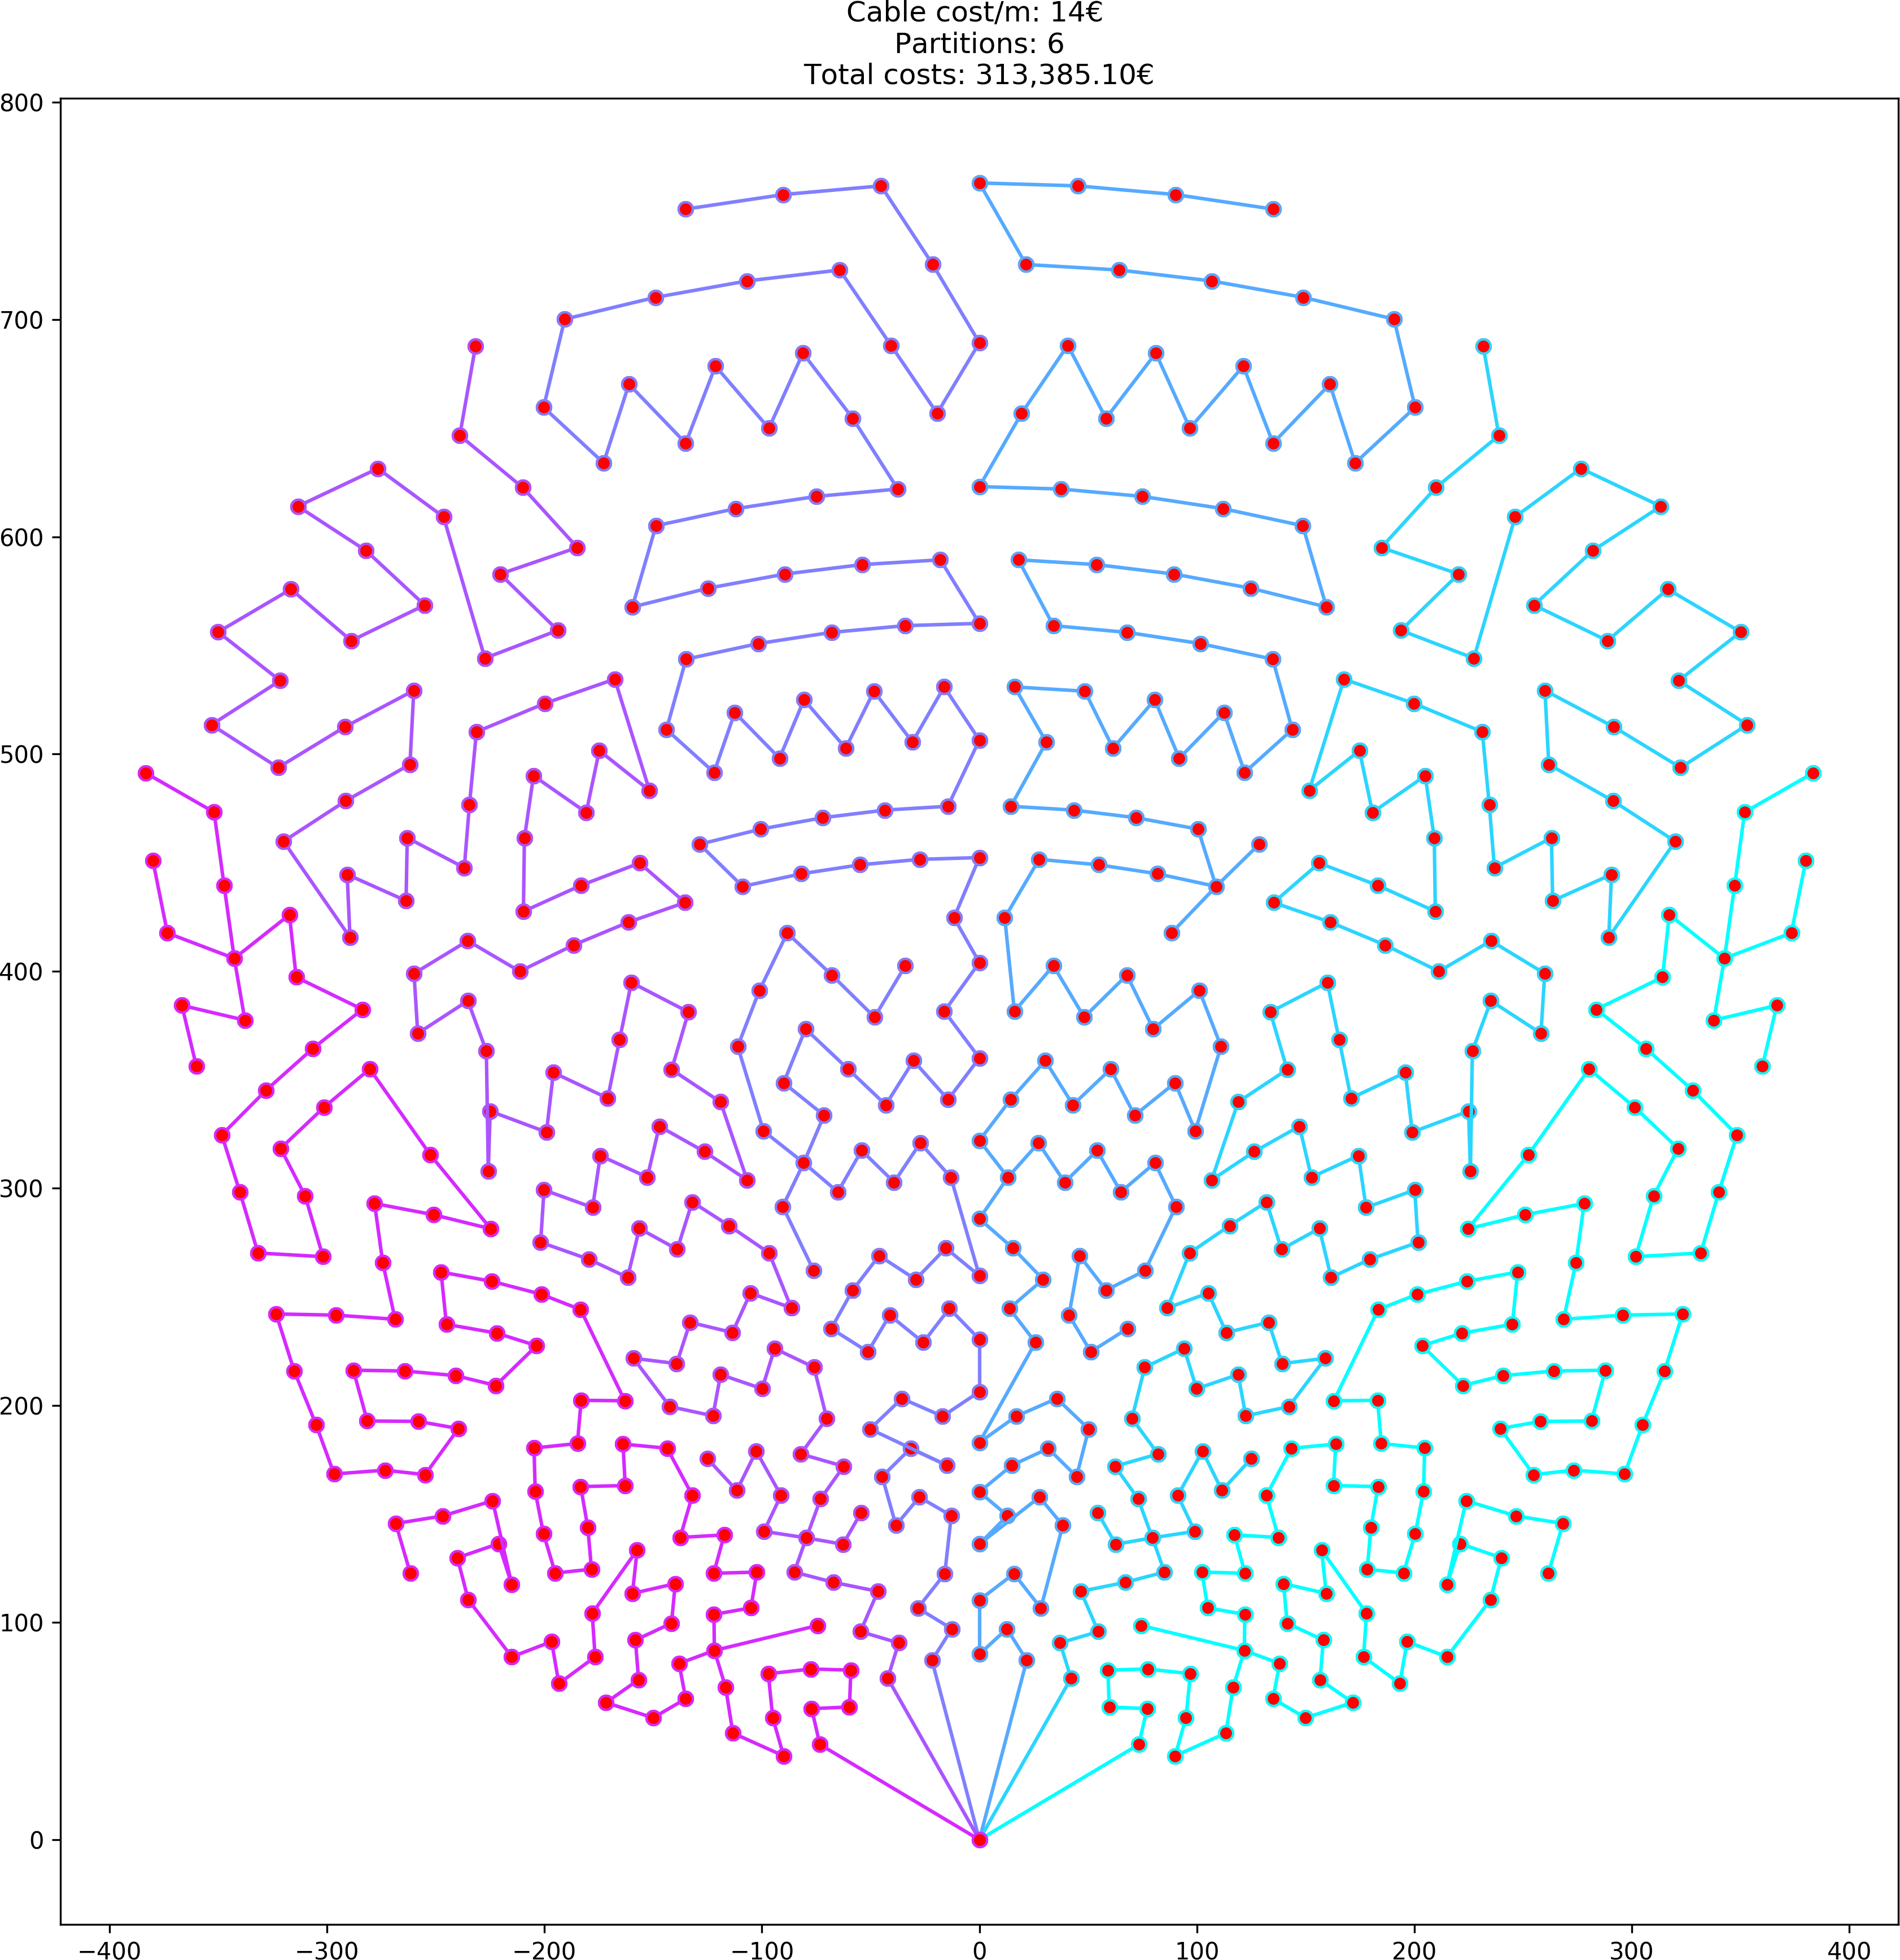
\includegraphics[width=0.75\textwidth]{./figs/output_mst_14_6.png}
    \caption{After local search for spanning trees. Total costs: 313,385.10\euro.}
  \end{figure}
\end{frame}

